\chapter{\IfLanguageName{dutch}{Proof-of-concept}{Proof-of-concept}}%
\label{ch:proof-of-concept}
\section{\IfLanguageName{dutch}{Virtuele omgeving}{Virtual environment}}%
\label{sec:Virtuele_omgeving}

Voor het opzetten van een oplossing en deze te kunnen testen en evalueren, is er een virtuele omgeving opgezet.
Deze virtuele omgeving is opgezet in GNS3, een netwerkemulator die het mogelijk maakt om netwerkapparatuur alsook virtuele machines te simuleren.
Binnen deze virtuele omgeving zal er aan netwerksegmentatie gedaan worden, het netwerk zal opgedeelde worden in 3 segmenten: een Admin, DMZ en employee segment.

\begin{figure}
  \centering
  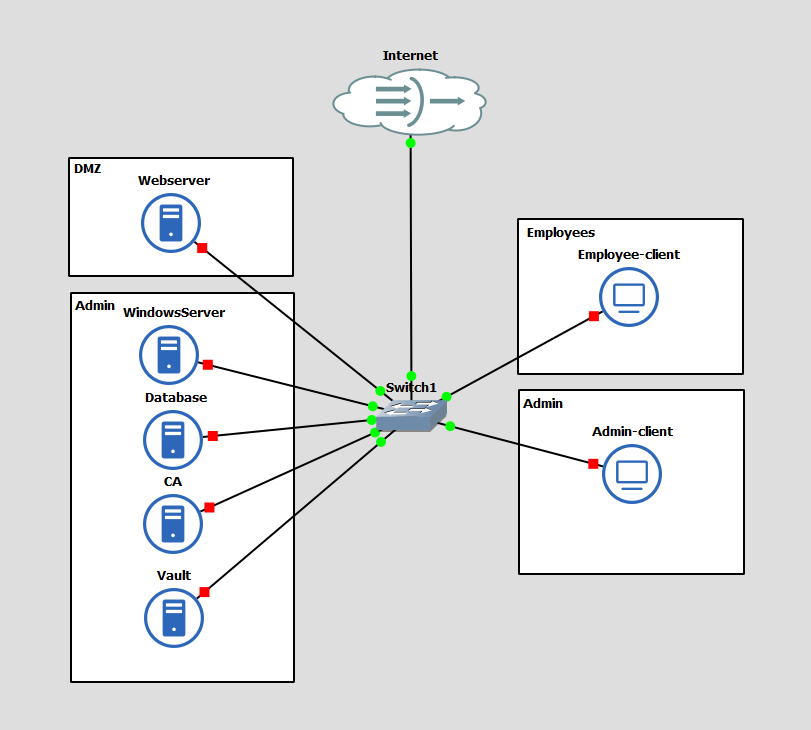
\includegraphics[width=1\textwidth]{Architectuurplan.png}
  \caption[Netwerkplan voor de proof-of-concept omgeving]{\label{fig:poc} De opzet van de proof-of-concept omgeving.}
\end{figure}


% Binnen het Admin segment zullen grotendeels van de servers staan alsook een workstation, in het DMZ segment zal er 1 server staan en in het employee segment zullen de werkstations staan.
% Deze segmentatie bestaat met als doel om het aantal vertrouwde root certificaten te beperken tot de benodigdheden van de verschillende segmenten, zo worden er minder root certificaten vertrouwd door de verschillende segmenten wat tot lagere security risico's leidt.
% Binnen het Admin segment staan er 4 servers, ``Windowsserver'', ``Database'', ``CA'' en ``Vault'' alsook is hier een workstation ``Admin-client''. Het DMZ segment heeft een server ``Webserver'' en het employee segment heeft 1 workstation ``Employee-client''. \\

\begin{table}
  \centering
  \begin{tabular}{lcr}
    \toprule
    \textbf{Naam} & \textbf{Netwerksegment} & \textbf{OS} & \textbf{Rollen} \\
    \midrule
    Webserver         & DMZ          & Ubuntu 22.04             & (Webserver, Chef infra client)                \\
    WindowsServer     & Admin        & Windows server 2022      & (Active directory, DNS server, SCCM server)               \\
    Database          & Admin        & Almalinux 8.8            & (Chef workstation, Chef infra client)                \\
    CA                & Admin        & Almalinux 8.8            & (Ansible control node, Chef infra server)                \\
    Vault             & Admin        & Ubuntu 22.04             & (Vault server)                \\
    Employee-client   & Employee     & Windows 11 Enterprise    & (SCCM Agent)           \\
    Admin-client      & Admin        & Windows 11 Enterprise    & (SCCM Agent)           \\
    \bottomrule
  \end{tabular}
  \caption[Oplijsten van machines in de POC omgeving]{\label{tab:POC_machines}Tabel met alle machines in de proof-of-concept omgeving.}
\end{table}

\pagebreak

\subsection{\IfLanguageName{dutch}{CA}{CA}}
\label{subsec:CA}

De CA server draait een Almalinux 8.8 image en is een Certificate Authority (CA). Deze CA zal de rol van interne CA spelen met een root certificaat dat gemaakt is met OpenSSL en ondertekend door de CA zelf. Naast de self-signed certificate zal er ook een leaf certificate gemaakt worden voor de webserver binnen deze omgeving.
Deze server zal ook de Ansible control node zijn voor de eerste oplossing, voor de tweede gevonden oplossing zal deze de rol van de Chef infra server innemen.

\subsection{\IfLanguageName{dutch}{Webserver}{Webserver}}
\label{subsec:Webserver}

De webserver draait op Ubuntu 22.04 en heeft een Nginx webserver draaien met een certificaat dat ondertekend werd door de eerder vermelde CA server.
Het doel van deze webserver is om de functionaliteit van het aanpassen van de truststore te testen, als een end-point de webpagina kan bereiken zonder waarschuwing via het https protocol, dan betekent dat de server ``CA'' zijn root certificaat aanwezig is in de end-point zijn truststore. \\
De server zal later ook de rol van Chef infra client spelen om te kunnen communiceren met de Chef infra server, daarnaast draait ook Hashicorp Vault Agent op deze server voor communicatie met de Vault server in de tweede oplossing.

\subsection{\IfLanguageName{dutch}{Windows server}{Windows server}}
\label{subsec:Windows_server}

Deze server draait Windows Server 2022 en is de domein controller van de virtuele omgeving. Het domein is ``Bachelorproef.local'' en de server heeft een Active Directory (AD) opgezet. De Active Directory bevat 2 logins voor de Windows clients ``Employee-client'' en ``Admin-client''. Binnen de AD zal elke Windows client die het netwerk betreedt automatisch gestoken worden. 
Deze clients worden manueel in de juiste organisational unit (OU) gestoken. In dit geval zijn dit de OU ``Employee'' en ``Admin''.
De Windows server heeft ook SCCM (System Center Configuration Manager) draaien die later in het onderzoek voor de tweede oplossing gebruikt zal worden om de truststores van de Windows clients te beheren.

\subsection{\IfLanguageName{dutch}{Vault}{Vault}}
\label{subsec:Vault}

De Vault server draait ook Ubuntu 22.04 en heeft een Hashicorp Vault server draaien. Deze Vault server zal gebruikt worden in de tweede oplossing om de root certificaten op een centrale plaats op te slaan.

\subsection{\IfLanguageName{dutch}{Employee-client}{Employee-client}}
\label{subsec:Employee-client}

Deze Windows client draait Windows 11, en bevindt zich in het Employee netwerksegment. Deze client maakt deel uit van het domein ``Bachelorproef.local'' en is ook lid van de OU ``Employee''.
Voor de tweede oplossing zal deze ook SCCM agent draaien.

\subsection{\IfLanguageName{dutch}{Admin-client}{Admin-client}}
\label{subsec:Admin-client}

Deze Windows client draait ook Windows 11 en bevindt zich in het Admin netwerksegment. Deze client maakt ook deel uit van het domein ``Bachelorproef.local'' en is ook lid van de OU ``Admin''.
Deze client draait ook SCCM agent bij de tweede oplossing.

\section{\IfLanguageName{dutch}{Voorbereiding truststores}{Preparing truststores}}%
\label{sec:Preparing_truststores}
Zoals ondervonden in de literatuurstudie, is het belangrijk om onnodige root certificaten te verwijderen uit de default truststores die bij installatie van de besturingssystemen zijn meegeleverd. Binnen deze proof-of-concept omgeving zijn er 3 verschillende systeem truststores, 1 voor de Windows end-points en 1 voor Ubuntu en Almalinux end-points.
Het is mogelijks een goed idee om eerst deze truststores te back-uppen vooraleer deze aan te passen, moest een probleem optreden op een later moment kan de truststore teruggezet worden naar de originele staat. \\

In Windows zijn de root certificaten opgeslagen in de ``Trusted Root Certification Authorities'' store. Om certificaten te verwijderen uit deze store, kan er gebruik gemaakt worden van de ``certlm.msc'' tool of het volgende PowerShell commando met als voorbeeld een root certificaat met de naam ``untrusted'':
\begin{minted}{powershell}
    Get-ChildItem -Path Cert:\LocalMachine\Root | Where-Object { $_.Subject -like "*untrusted*" } | Remove-Item
\end{minted}
\\

Ubuntu werkt met een config file die zich bevindt in de directory ``/etc/ca-certificates.conf''. Deze file bevat een lijst van root certificaten die vertrouwd worden door het systeem. Om root certificaten te verwijderen uit deze file, kunnen deze lijnen verwijderd of gecommentarieerd worden.
Wanneer het commando ``update-ca-certificates'' uitgevoerd wordt, worden de root certificaten die in deze file staan, samen met de root certificaten die in de directory ``/usr/local/share/ca-certificates'' staan, samengevoegd in de truststore van het systeem. Deze truststore is simpelweg een file die de bundle met root certificaten bevat. 
Dit bestand kan gevonden worden in de directory ``/etc/ssl/certs/ca-certificates.crt''. \\

Na het aanpassen van de config file kan het ca-certificates.crt bestand verwijderd worden en kan het commando ``update-ca-certificates'' uitgevoerd worden om de truststore opnieuw aan te maken als volgt:
\begin{minted}{bash}
    sudo rm /etc/ssl/certs/ca-certificates.crt
    sudo update-ca-certificates --fresh
\end{minted}
Het is hierbij dan ook belangrijk om te weten dat de certificaten uit /usr/local/share/ca-certificates toegevoegd worden aan deze truststore, deze directory is standaard leeg, moest hier een certificaat staan, zal dit certificaat ook toegevoegd worden aan de truststore. \\

In Almalinux zitten de root certificaten in verschillende bundle files in directories per applicaties. Deze directory is ``/etc/pki/ca-trust/extracted/'', binnenin deze directory liggen dan meerdere subdirectories benaamd naar de bijhorende applicatie die elk een bundle file bevatten, hieruit moeten de onnodige certificaten verwijderd worden. \\

Om deze aan te passen moet er eigenlijk maar slechts 1 bestand aangepast worden. De file /etc/pki/tls/certs/ca-bundle.crt bevat de root certficaten die standaard vertrouwd worden en deze inhoud wordt bij de uitvoer van het commando ``update-ca-trust'' toegevoegd aan de bundle file in elke subdirectory.
Elk certificaat heeft zijn naam in commentaar vorm staan, om een certificaat te verwijderen kan de lijn met de CA naam tot en met de eerst volgende lijn met ``-----END CERTIFICATE-----'' verwijderd worden.
Zoals bij ubuntu is het belangrijk om te weten dat als het commando ``update-ca-trust'' uitgevoerd wordt, de root certificaten die in de directory ``/etc/pki/ca-trust/source/anchors/'' staan ook toegevoegd worden aan alle truststores van al de applicaties. Deze zou normaal ook standaard leeg moeten zijn. \\

Voor de gevonden oplossingen werden alle certificaten uit de default truststores verwijderd, alle nodige certificaten kunnen via de oplossingen terug toegevoegd worden aan de truststores. Dit zorgt ervoor dat de default truststores nooit meer aangeraakt moeten worden en enkel de certificaten binnen de oplossing zelf moeten beheerd worden.
Een belangrijke observatie tijdens het uitvoeren van dit onderzoek was dat zowel Windows als Linux minimum 1 certificaat moeten hebben in hun truststore, Windows zal het verwijderen van het allerlaatste certificaat niet toelaten en Applicaties binnen Linux zullen foutmeldingen geven wanneer hun bijhorende bundle file niet bestaat en/of leeg is. \\

\pagebreak

\section{\IfLanguageName{dutch}{Eerste oplossing}{First solution}}%
\label{sec:Eerste_oplossing}

\begin{figure}
  \centering
  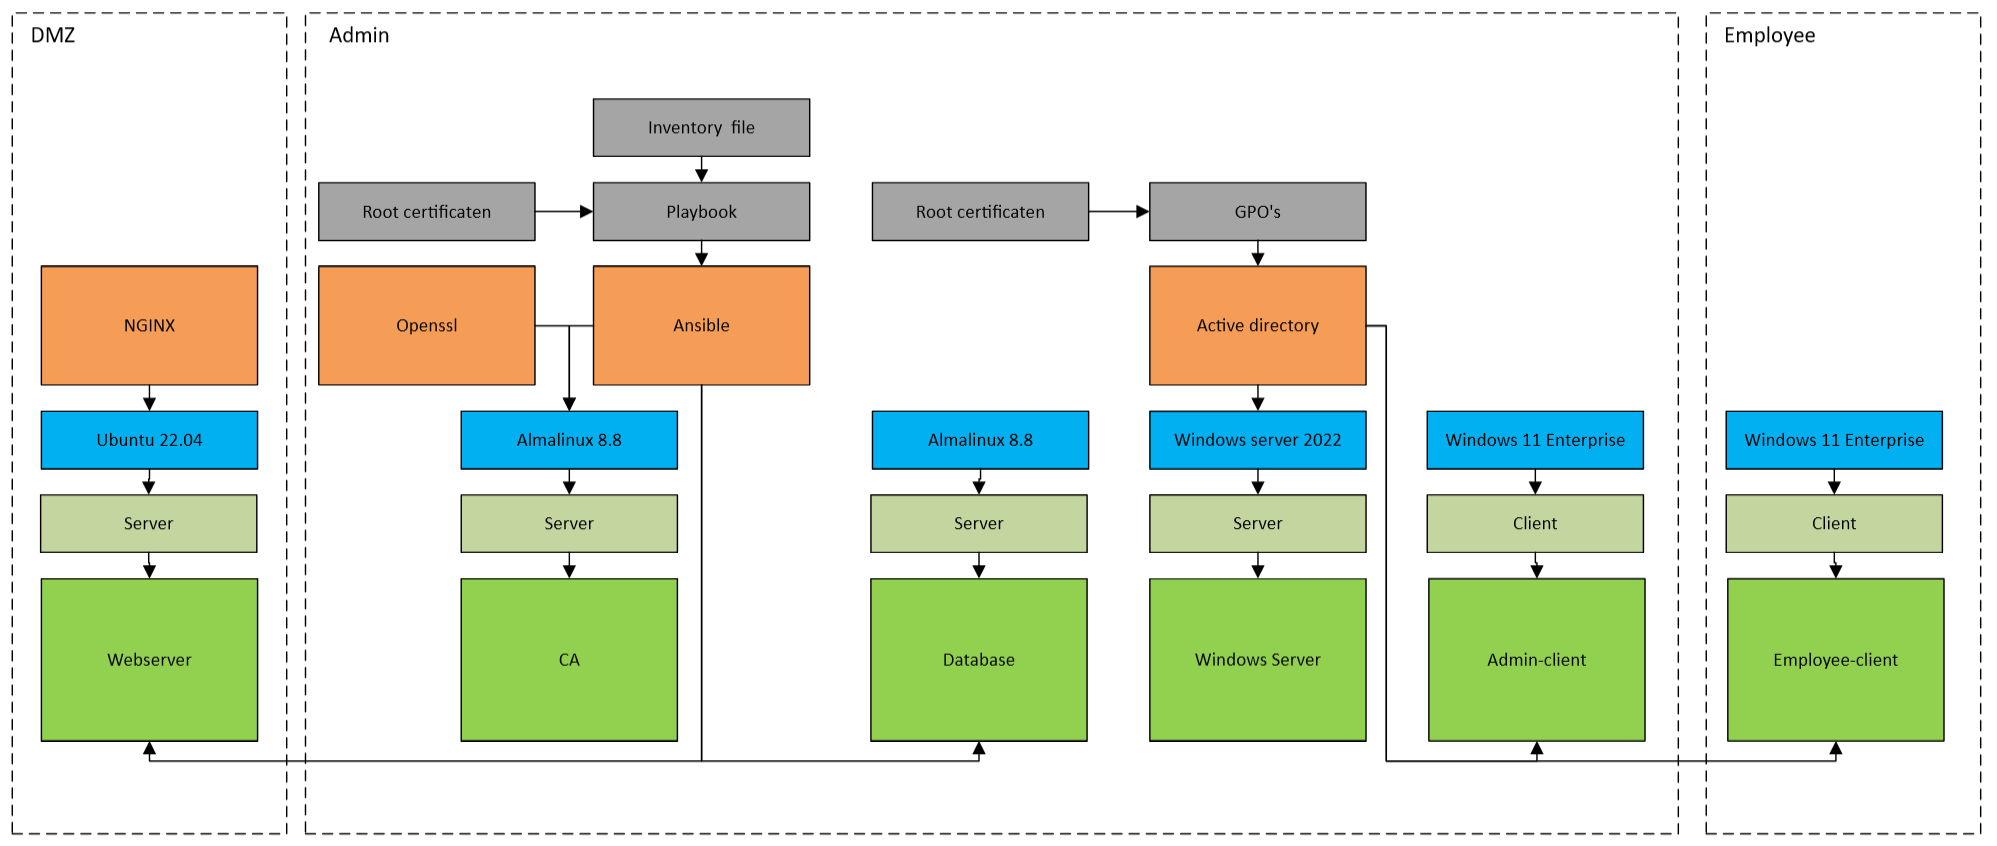
\includegraphics[width=1\textwidth]{Architectuurplan_opl1.png}
  \caption[Architectuurplan van de eerste oplossing]{\label{fig:opl1} Het architectuurplan van de werking van de eerste oplossing.}
\end{figure}

De initieel gevonden oplossing bestond uit het gebruik van Ansible voor de Linux end-points en Group Policy Objects (GPO's) voor de Windows end-points. Beide de Windows server en CA server (die de Ansible control server is) hebben een kopie van de root certificaten die bij de Windows kant in de GPO's worden gestoken en bij de Linux kant overgezet worden via Ansible.

\subsection{\IfLanguageName{dutch}{Oplossing door middel van GPO's met root certificaten}{Solution for Windows end-points using GPOs with root certificates}}
\label{subsec:Oplossing_door_middel_van_GPOs_met_root_certificaten}
Om Windows clients hun truststores centraal te kunnen beheren, kan er simpelweg een GPO (Group Policy Object) aangemaakt worden die root certificaten bevat en deze kan dan toegepast worden op een organizational unit (OU) binnen de Active Directory.
Er kan dus een GPO aangemaakt worden per OU (in dit geval de 3 OU's voor de 3 netwerksegmenten) die elk de juiste root certificaten bevatten. \\

Voor deze proof of concept zal er een verzameling van root certificaten opgeslagen worden in een directory op de Windows server, deze directory zal 3 subdirectories bevatten, 1 voor elk netwerksegment. De root certificaten die in deze subdirectories staan zijn de root certificaten die de clients in dat netwerksegment moeten vertrouwen.
De GPO's zullen dan de root certificaten uit deze subdirectories halen en deze toevoegen aan de truststore van de clients in dat netwerksegment. \\

De GPO's kunnen als volgt aangemaakt worden:
\begin{itemize}
    \item Open de Group Policy Management Console (GPMC) op de Windows server.
    \item Maak een nieuwe GPO aan door met de rechtermuisknop op de OU te klikken en ``Create a GPO in this domain, and Link it here'' te selecteren.
    \item Geef de GPO een naam, bijvoorbeeld ``Employee-certificates''.
    \item Klik met de rechtermuisknop op de GPO en selecteer ``Edit''.
    \item Ga naar Computer Configuration > Policies > Windows Settings > Security Settings > Public Key Policies > Trusted Root Certification Authorities.
    \item Klik met de rechtermuisknop en selecteer ``Import''.
    \item Volg de wizard om het root certificaat te importeren vanuit de directory op de Windows server.
    \item Herhaal deze stappen voor de andere OU's en root certificaten.
\end{itemize}

De GPO's kunnen dan toegepast worden, dit kan door met de rechtermuisknop op de OU te klikken en ``Link an Existing GPO'' te selecteren. Selecteer dan de GPO die je wilt toepassen op de OU. Daarna moet de policy nog enforced worden door met de rechtermuisknop op de GPO te klikken en ``Enforce'' te selecteren. Dit zorgt ervoor dat de GPO ook toegepast wordt op de OU en alle sub-OU's die binnen deze OU zitten. \\

Op de clients kan je dan de GPO's toepassen door het volgende commando uit te voeren in de command prompt:
\begin{minted}{powershell}
    gpupdate /force
\end{minted}
Ook kan de GPO toegepast worden door de clients opnieuw op te starten. 

\pagebreak

\subsection{\IfLanguageName{dutch}{Oplossing voor Linux end-points met Ansible}{Solution for Linux end-points using Ansible}}
\label{subsec:Oplossing_voor_Linux_end-points_met_Ansible}

Om het probleem van het centraal beheren van de root certificaten op te lossen, kan er voor de Linux end-points een Ansible playbook gemaakt worden dat root certificaten kan toevoegen aan de truststores.
De CA server zal in deze proof-of-concept ook de Ansible control server zijn. Dit is de server die de Ansible playbooks zal uitvoeren op de end-points via SSH connecties.
Hiervoor is een inventory bestand nodig dat de IP adressen of domein naam van de end-points bevat samen met de gebruiker die gebruikt zal worden voor de SSH verbinding en de waar de public key die gebruikt wordt door de Ansible node ligt. Dit bestand voor deze omgeving ziet er als volgt uit: \\

\begin{listing}[H]
    \begin{minted}[caption={Ansible inventory file},label={lst:inventory_file}]{yaml}
        [DMZ]
        web ansible_host=bpweb.bachelorproef.local ansible_user=ubuntu ansible_ssh_private_key_file=/home/almlainux/.ssh/id_rsa

        [Admin]
        db ansible_host=db.bachelorproef.local ansible_user=almalinux ansible_ssh_private_key_file=/home/almalinux/.ssh/id_rsa
        ca ansible_host=ca.bachelorproef.local ansible_user=almalinux ansible_ssh_private_key_file=/home/almalinux/.ssh/id_rsa
    \end{minted}
    \caption[Inventory file voor Ansible]{Het gebruikte inventory bestand voor Ansible.}
\end{listing}

Net zoals bij de Windows server zal er een directory aangemaakt worden op de server ``CA'' die subdirectories bevat voor elk netwerksegment. Deze subdirectories bevatten de root certificaten die de end-points in dat netwerksegment moeten vertrouwen.
Met deze bestanden en directories kan er een Ansible playbook gemaakt worden dat de root certificaten uit de juiste subdirectory haalt en toevoegt aan de truststore van de end-points. Dit kan gedaan worden met het volgende Ansible playbook:
\begin{listing}[H]
\begin{minted}{yaml}
- name: truststore update
  hosts: all
  become: true
  vars:
    cert_source_dir: >-
      {{ '/home/almalinux/Ansible/DMZ' if 'DMZ' in group_names else '/home/almalinux/Ansible/Admin' }}
    dest_cert_dir: >-
      {{ '/usr/local/share/ca-certificates' if ansible_os_family == "Debian" else '/etc/pki/ca-trust/source/anchors' }}
    update_command: >-
      {{ 'update-ca-certificates' if ansible_os_family == "Debian" else 'update-ca-trust extract' }}

  tasks:

    ### LEDIGEN DIRECTORIES ###
    - name: verwijderen van truststore directory
      file:
        path: "{{ dest_cert_dir }}"
        state: absent
      when: ansible_os_family in ["Debian", "RedHat"]

    - name: de truststore directory opnieuw aanmaken
      file:
        path: "{{ dest_cert_dir }}"
        state: directory
        owner: root
        group: root
        mode: '0755'
      when: ansible_os_family in ["Debian", "RedHat"]

    ### CERTIFICATEN INSTALLEREN ###
    - name: Kopieer certificaten van Ansible control node naar de truststore directory op end-point
      copy:
        src: "{{ cert_source_dir }}/"
        dest: "{{ dest_cert_dir }}/"
        owner: root
        group: root
        mode: '0644'
        remote_src: no

    ### TRUST STORE UPDATEN ###
    - name: Update systeem truststore
      command: "{{ update_command }}"


\end{minted}
\caption[Ansible playbook]{De Ansible playbook die certificaten van de Ansible control node naar de end-point truststore directory kopieert.}
\end{listing}

\begin{listing}[H]\ContinuedFloat
\begin{minted}{yaml}
    ### DEBUG ###
    - name: Bevestiging
      debug:
        msg: "Alle truststores zijn up-to-date"
\end{minted}
\caption[]{De Ansible playbook die certificaten van de Ansible control node naar de end-point truststore directory kopieert.}
\end{listing}

De playbook begint met het aanmaken van 3 variabelen, de eerste variabele ``cert\_source\_dir'' bevat de directory waar de root certificaten staan die de end-point moet vertrouwen, deze directory is afhankelijk van de groep waar de end-point in zit binnen de inventory file.
Als tweede variabele ``dest\_cert\_dir'' wordt de directory bepaald waar de root certificaten naartoe gekopieerd worden, deze directory is afhankelijk van de linux distributie van de end-point.
De laatste variabele ``update\_command'' bevat het commando dat gebruikt zal worden om de truststore te updaten, dit is ook afhankelijk van de linux distributie. \\

Deze playbook zal hierna de truststore directory ledigen door het simpelweg te verwijderen, dit is opzich geen probleem want alle certificaten zijn momenteel nogsteeds aanwezig in de truststore bundle files van de applicaties.
Vervolgens zal deze directory weer aangemaakt worden met de juiste permissies en hierna zullen de root certificaten uit de juiste bron directory gekopieerd worden naar de juiste doel directory.
Als laatste zal de truststore geüpdatet worden met het correcte commando afhankelijk van de linux distributie. Hierbij zullen de root certificaten in de bundle files van de applicaties gestoken worden. \\

Een belangrijke opmerking bij deze playbook is dat het alleen zal uitgevoerd worden voor Ubuntu en Red Hat end-points, de stappen zullen overgeslagen worden voor andere distributies. 
Voor andere distributies moet er een juiste aanwijzing van variabelen voorzien worden alsook moeten deze vermeld worden onder elke stap in de playbook binnen het 'when' veld. \\

Om het voorgaande Ansible playbook uit te voeren, kan er gebruik gemaakt worden van de volgende commando's:
\begin{minted}{bash}
    ansible-playbook -i inventory playbook.yml
\end{minted}

Waarbij ``inventory'' het inventory bestand is dat de IP adressen van de end-points bevat en ``playbook.yml'' het bovenstaande Ansible playbook is.

\pagebreak

\subsection{\IfLanguageName{dutch}{Pro's en Con's van de eerste oplossing}{Pro's and Con's of the first solution}}
\label{subsec:Pros_en_Cons_van_de_eerste_oplossing}
\begin{itemize}
    \item Pro's:
    \begin{itemize}
        \item De root certificaten kunnen eenvoudig beheerd worden binnen de Ansible node en Windows server directory.
        \item Geen nodige installatie van extra software op de end-points.
        \item End-points ondervinden geen hinder van de installatie van de root certificaten.
        \item Er zijn weinig points of failure aangezien de oplossing geen bijkomende servers of software nodig heeft.
    \end{itemize}
    \item Con's:
    \begin{itemize}
        \item De GPO's passen alleen maar toe wanneer de end-points opnieuw opgestart worden of de GPO's geforceerd worden.
        \item Er is geen directe functie voor het importeren van certificaten in een GPO via Powershell, dit betekent dat als er veel root certificaten zijn, het handmatig aanmaken van de GPO's tijdrovend zal zijn.
        \item De certificaten staan in directories die niet beveiligd zijn, dit brengt een risico mee dat de certificaten binnen de directory kunnen worden aangepast of verwijderd.
        \item Zowel de Windows server als de CA server (de Ansible control server) hebben een kopie van de root certificaten, bij een aanpassing van de root certificaten moeten deze op beide servers aangepast worden.
        \item De Ansible playbook is niet schaalbaar, een server maakt SSH verbindingen met de end-points en voert de playbook uit op elke end-point. Dit betekent dat als er veel end-points zijn, de Ansible playbook traag zal zijn en mogelijk niet alle end-points kan bereiken.
    \end{itemize}
\end{itemize}

\pagebreak

\section{\IfLanguageName{dutch}{Tweede oplossing}{Second solution}}%
\label{sec:Tweede_oplossing}

\begin{figure}
  \centering
  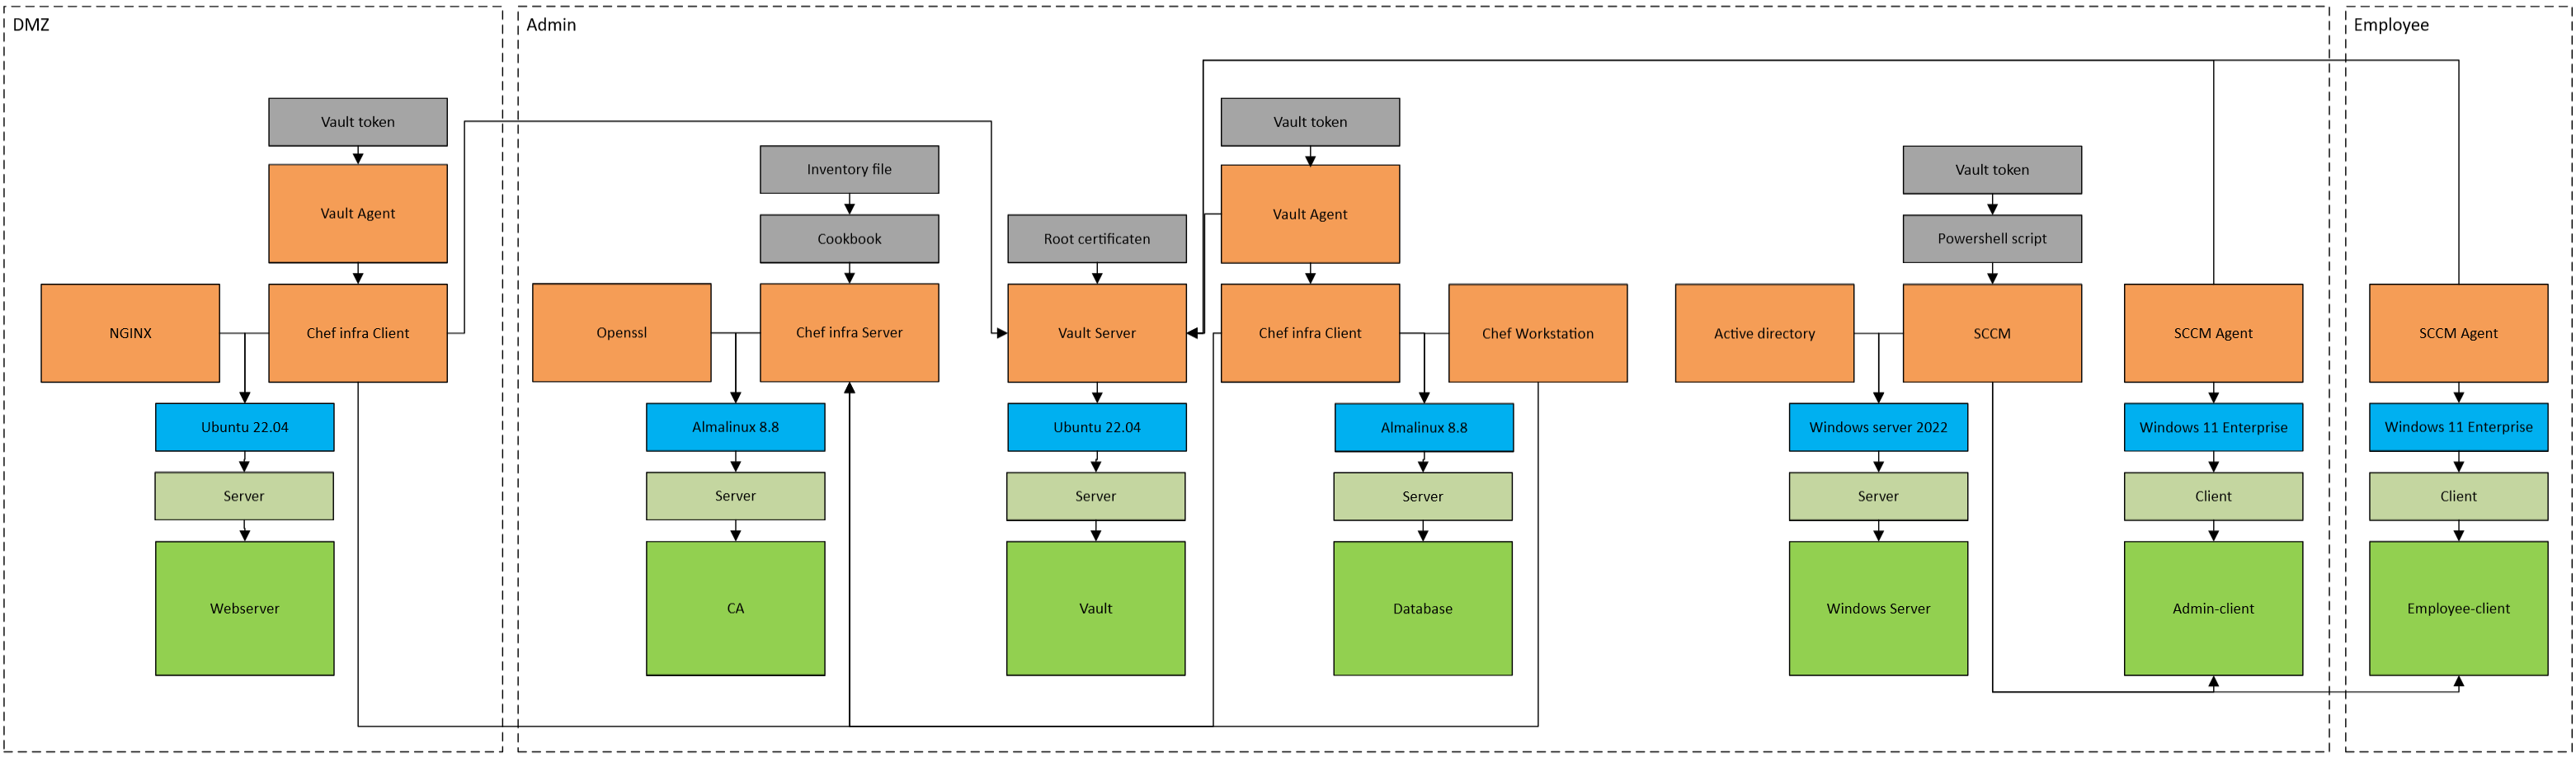
\includegraphics[width=1\textwidth]{Architectuurplan_opl2.png}
  \caption[Architectuurplan van de tweede oplossing]{\label{fig:opl2} Het architectuurplan van de werking van de tweede oplossing.}
\end{figure}

De tweede oplossing streeft ernaar de negatieve punten van de eerste oplossing te verhelpen. In de tweede oplossing zal er een Hashicorp Vault server gebruikt worden om root certificaten centraal op te slaan en deze te beheren. 
Hiervoor zal op de Linux end-points een Hashicorp Vault agent moeten draaien voor toegang te krijgen tot de Vault server met een token, op de Windows server zal er centraal een token aanwezig zijn voor alle Windows end-points.
Aan de Windows kant van de oplossing zal er een System Center Configuration Manager (SCCM) server gebruikt worden om een Powershell script te deployen op de end-points die de juiste root certificaten uit de Vault server haalt en deze toevoegt aan de truststore.
Voor de Linux end-points zal er hier in de plaats van Ansible een Chef infra server gebruikt worden die de instructies aan end-points aanbied om de certificaten uit de Vault server te halen en deze toe te voegen aan de truststore.

\subsection{\IfLanguageName{dutch}{Installeren van een Vault server}{Installing a Vault server}}
\label{subsec:Installeren_van_een_Vault_server}

Om het probleem van het dubbel beheren van de root certificaten op te lossen, moet er een centraal punt op het netwerk zijn die de root certificaten bevat. Dit kan gedaan worden door een Hashicorp Vault server op te zetten. Deze server brengt naast het beheren van de root certificaten ook autorisatie met zich mee waardoor de certificaten ook beveiligd zijn.\\
Binnen deze proof-of-concept omgeving is er een standalone server voorzien voor de Hashicorp Vault genaamd ``Vault''. 
Deze server heeft een kopie van de directories met root certificaten die op de servers ``CA'' en ``Windows Server'' stonden. Daarnaast zal Vault in ``dev'' mode draaien, dit is een testmodus die het mogelijk maakt om snel te experimenteren met Vault zonder dat er een volledige configuratie nodig is. 
In deze modus zal de vault server ook geen persistentie hebben, wat betekent dat alle gegevens uit de vault verloren gaan als de vault sluit of de server stopt.

%De vault server kan gedownload worden van de Hashicorp website, de server kan gedownload worden met het volgende commando:
%\begin{minted}{bash}
%    wget -O - https://apt.releases.hashicorp.com/gpg | sudo gpg --dearmor -o /usr/share/keyrings/hashicorp-archive-keyring.gpg
%    echo "deb [arch=$(dpkg --print-architecture) signed-by=/usr/share/keyrings/hashicorp-archive-keyring.gpg] https://apt.releases.hashicorp.com $(lsb_release -cs) main" | sudo tee /etc/apt/sources.list.d/hashicorp.list
%    sudo apt update && sudo apt install vault
%\end{minted}

De vault server wordt opgestart met de volgende commando:
\begin{minted}{bash}
    vault server -dev -dev-listen-address="0.0.0.0:8200"
\end{minted}

Dit maakt de Vault server toegankelijk op all zijn IP adressen van de server op poort 8200. \\
De Vault server zal onderverdelingen hebben per netwerksegment, binnen elk netwerksegment zullen de root certificaten staan. Naast de root certificaten zal er ook een manifest binnen elk netwerksegment bestaan die een oplijsting bevat van zijn root certificaten. 
Deze manifest kan gebruikt worden door end-points om elk root certificaat binnen hun netwerksegment op te halen. \\

Voor het aanmaken van de indelingen en manifests werd er een bash script gemaakt die de root certificaten uit de directories haalt en deze toevoegt aan de vault. Dit script ziet er als volgt uit:
\begin{listing}[H]
\begin{minted}{bash}
#!/bin/bash

VAULT_ADDR="http://127.0.0.1:8200"
export VAULT_ADDR

BASE_CERT_DIR="/home/ubuntu/"
SEGMENTS=("DMZ" "Admin" "Employee")

for SEGMENT in "${SEGMENTS[@]}"; do
    SEGMENT_DIR="$BASE_CERT_DIR/$SEGMENT"
    VAULT_PATH="secret/certs/$SEGMENT"

    echo "certificaten uploaden voor segment: $SEGMENT"

    # Remove the existing manifest and its metadata
    echo " - verwijderen van manifest en metadata voor $SEGMENT"
    vault kv delete "$VAULT_PATH/_manifest" || echo "geen manifest te verwijderen"
    vault kv metadata delete "$VAULT_PATH/_manifest" || echo "geen metadata te verwijderen"

    # certificaten uploaden van de directory
    for cert_file in "$SEGMENT_DIR"/*.pem "$SEGMENT_DIR"/*.crt; do
        [ -e "$cert_file" ] || continue  # Skip if no matching files
        cert_name=$(basename "$cert_file" | sed 's/\.[^.]*$//')  # extentie verwijderen

        echo " - Uploading $cert_name from $cert_file"
        vault kv put "$VAULT_PATH/$cert_name" cert=@"$cert_file"
    done

    # niew manifest maken (lijst van certs) voor fetching op end-points
    echo "manifest maken voor $SEGMENT"
    cert_keys=$(ls "$SEGMENT_DIR" | sed 's/\.[^.]*$//' | jq -R . | jq -s .)
    vault kv put "$VAULT_PATH/_manifest" keys="$cert_keys"
done

echo "Alle certs geupload naar de Vault."
\end{minted}
\caption[Bash script voor het uploaden van certificaten naar de Vault]{Het bash script dat de root certificaten upload naar de Vault server.}
\end{listing}

Voor de beveiliging van de root certificaten in de vault zal er gebruik gemaakt worden van token autorisatie. Dit is een manier van autorisatie waarbij een token door de end-points wordt gebruikt om toegang te krijgen tot de vault.
Om ervoor te zorgen dat de rechten met deze token gelimiteerd zijn, kan er een policy aangemaakt worden. \\

De volgende policy kan gebruikt worden voor read-only toegang tot alle root certificaten op alle netwerksegmenten:
\begin{listing}[H]
\begin{minted}{hcl}     
    path "secret/data/certs/*" {
    capabilities = ["read", "list"]
    }

    path "secret/metadata/certs/*" {
    capabilities = ["read", "list"]
    }

    path "secret/data/certs/*/manifest" {
    capabilities = ["read"]
    }

    path "secret/data/certs/*/*" {
    capabilities = ["read"]
    }
\end{minted}
\caption[Policy met leesrechten tot de Vault]{De policy die leesrechten geeft tot de root certificaten in de Vault.}
\end{listing}

Deze policy kan dan toegevoegd worden aan een role en uiteindelijk kan een token aangemaakt worden met deze role.
Eerst moet approle, de manier van authenticatie aangezet worden met het volgende commando:

\begin{minted}{bash}
    vault auth enable approle
\end{minted}

Daarna kan de voorgaande policy aangemaakt worden met het volgende commando:

\begin{minted}{bash}
    vault policy write certs-read public-certs.hcl
\end{minted}

Waarbij ``public-certs.hcl'' het bestand is dat de policy bevat en ``certs-read'' de naam die gegeven wordt aan de policy. \\

De role kan dan aangemaakt worden als volgt:
\begin{minted}{bash}
    vault write auth/approle/role/chef_cert_reader \
    token_policies="certs-read" \
    secret_id_ttl="60m" \
    token_ttl="30m" \
    token_max_ttl="60m"
\end{minted}
Waarbij chef\_cert\_reader de naam is die gegeven wordt aan de role. Token\_policies linkt de policy die zojuist werd gemaakt aan de role, secret\_id\_ttl is de tijd dat de secret\_id geldig is, token\_ttl is de tijd dat de token geldig is en token\_max\_ttl is de maximale tijd dat de token geldig is.
Clients kunnen via de role\_id en secret\_id een token aanvragen, voor het bekomen van de role\_id kan er gebruik gemaakt worden van het volgende commando:

\begin{minted}{bash}
    vault read auth/approle/role/chef_cert_reader
\end{minted}

Deze role\_id blijft geldig tot en met de vault server opnieuw opgestart wordt. De secret\_id is ook nodig, deze kan aangemaakt worden met het volgende commando:
\begin{minted}{bash}
    vault write -f auth/approle/role/chef_cert_reader/secret-id
\end{minted}
De secret\_id heeft een bepaalde levensduur die eerder werd ingesteld bij het maken van de role.

\subsection{\IfLanguageName{dutch}{Installeren van een Vault agent}{Installing a Vault agent}}
\label{subsec:Installeren_van_een_Vault_agent}

Om de clients toegang te geven tot de vault, moet er een token aangemaakt worden met de role\_id en secret\_id waarover hiervoor werd gesproken. Om deze token aan te maken, moet er een vault agent draaien op de end-point.
Deze agent kan geconfigureerd worden met het volgende bestand '/etc/vault/agent-config.hcl':

\begin{listing}[H]
\begin{minted}{hcl}
pid_file = "/run/vault/vault-agent.pid"

vault {
  address = "http://vault.bachelorproef.local:8200"
}

auto_auth {
  method "approle" {
    mount_path = "auth/approle"
    config = {
      role_id_file_path   = "/var/lib/vault/role_id"
      secret_id_file_path = "/var/lib/vault/secret_id"
      remove_secret_id_file_after_reading = false
    }
  }

  sink "file" {
    config = {
      path = "/var/lib/vault/agent-token"
    }
  }
}

cache {
  use_auto_auth_token = true
}

listener "tcp" {
  address     = "0.0.0.0:8201"
  tls_disable = true
}
\end{minted}
\caption[De configuratie voor Vault Agent]{De gebruikte configuratie voor de Vault agent.}
\end{listing}

Waarbij ``role\_id\_file\_path'' het pad is naar het bestand dat de role\_id bevat en ``secret\_id\_file\_path'' het pad is naar het bestand dat de secret\_id bevat. 
Sink ``file'' zorgt ervoor dat de token die aangemaakt wordt door de agent, opgeslagen wordt in het bestand ``/var/lib/vault/agent-token''. Dit bestand kan dan gebruikt worden door de end-point om toegang te krijgen tot de vault. \\

Om de agent te starten kan er gebruik gemaakt worden van het volgende commando:
\begin{minted}{bash}
    vault agent -config=/etc/vault/agent-config.hcl
\end{minted}

De agent zal dan automatisch de token aanmaken en hernieuwen wanneer deze verloopt. \\

Ook op Windows kan Vault agent draaien als een service, helaas door de limitaties van bronnen voor deze proof-of-concept is de installatie hiervan niet uitgevoerd, in de plaats hiervan zal er een token aangemaakt worden in een shared directory op de Windows server.

\pagebreak

\subsection{\IfLanguageName{dutch}{Oplossing voor Windows end-points met SCCM en Vault}{Solution for Windows end-points using SCCM and Vault}}
\label{subsec:Oplossing_voor_Windows_end-points_met_SCCM_en_Vault}

Aangezien het importeren van root certificaten in de GPO's niet geautomatiseerd kan worden, is er geen schaalbaarheid in de vorige oplossing. Dit betekent dat als er veel root certificaten zijn, het handmatig aanmaken van de GPO's een grote kost in tijd zal zijn.
Om dit probleem op te lossen kan er in de plaats van root certificaten aan de GPO's te koppelen, een script gemaakt worden dat de root certificaten ophaalt en deze toevoegt aan de truststore van de clients. \\

Dit kan gedaan worden met het volgende PowerShell script:

\begin{listing}[H]
\begin{minted}{powershell}
param (
    [Parameter(Mandatory = $true)]
    [string]$NetworkSegment
)

# Configuration
$VaultAddress = "http://vault.bachelorproef.local:8200"
$LocalCertPath = "C:\Temp\VaultCerts"
$TokenFilePath = "\\bachelorproef.local\SYSVOL\bachelorproef.local\scripts\archive\token.txt"

# Logging
$LogFile = "C:\Temp\Truststore_Clear_And_Update_Log.txt"
function Write-Log {
    param (
        [string]$Message
    )
    $Timestamp = Get-Date -Format "yyyy-MM-dd HH:mm:ss"
    Add-Content -Path $LogFile -Value "$Timestamp - $Message"
}

Write-Log "Script started with NetworkSegment = $NetworkSegment"

# Step 1: Vault token ophalen van bestand
Write-Log "Vault token ophalen op locatie: $TokenFilePath..."



\end{minted}
\caption[Powershell script om root certificaten te importeren van de Vault]{Het Powershell script dat op end-points draait om root certificaten te importeren van de Vault server.}
\end{listing}

\begin{listing}[H]\ContinuedFloat
\begin{minted}{powershell}
try {
    if (-Not (Test-Path $TokenFilePath)) {
        Write-Log "Token file niet gevonden op: $TokenFilePath. Exiting..."
        exit
    }
    $VaultToken = Get-Content -Path $TokenFilePath -ErrorAction Stop
    Write-Log "Vault token succesvol opgehaald"
} catch {
    Write-Log "Kan vault token niet ophalen: $($_.Exception.Message). Exiting..."
    exit
}

# Ensure local cert path exists
New-Item -ItemType Directory -Force -Path $LocalCertPath | Out-Null

# Step 2: Clear Truststore
Write-Log "truststore clearen..."
$Certs = Get-ChildItem -Path Cert:\LocalMachine\Root
foreach ($Cert in $Certs) {
    try {
        Remove-Item -Path $Cert.PSPath -Force
        Write-Log "certificaat verwijderd: $($Cert.Subject)"
    } catch {
        Write-Log "Kon certificaat niet verwijderen: $($Cert.Subject). Error: $($_.Exception.Message)"
    }
}
Write-Log "Truststore cleared."

# Step 3: root certs van vault ophalen

$ManifestUrl = "$VaultAddress/v1/secret/data/certs/$NetworkSegment/_manifest"
try {
    $Manifest = Invoke-RestMethod -Uri $ManifestUrl -Headers @{ "X-Vault-Token" = $VaultToken } -Method GET
    Write-Log ("Fetched manifest voor segment $NetworkSegment : " + ($Manifest | ConvertTo-Json -Depth 3))
}

\end{minted}
\caption[]{Vervolg op het Powershell script.}
\end{listing}

\begin{listing}[H]\ContinuedFloat
\begin{minted}{powershell}
catch {
    $msg = $_.Exception.Message
    Write-Log "Kon manifest niet fetchen voor '$NetworkSegment': $msg"
    exit
}

# structuur van de manifest controlleren
if ($Manifest.data -and $Manifest.data.data) {
    try {
        $CAList = $Manifest.data.data.keys | ConvertFrom-Json
    }
    catch {
        Write-Log "kon manifest niet parsen naar JSON voor '$NetworkSegment'. Exiting..."
        exit
    }
} else {
    Write-Log "Foutief manifest formaat of geen certificaten gevonden voor '$NetworkSegment'. Exiting..."
    exit
}

if ($CAList.Count -eq 0) {
    Write-Log "Geen certificaten gevonden voor '$NetworkSegment'. Exiting..."
    exit
}

foreach ($CA in $CAList) {
    if ([string]::IsNullOrWhiteSpace($CA)) {
        Write-Log "Lege CA naam gevonden in manifest. overslaan..."
        continue
    }

    $CertUrl = "$VaultAddress/v1/secret/data/certs/$NetworkSegment/$CA"
    Write-Log "Downloading cert: $CA"


    

\end{minted}
\caption[]{Vervolg op het Powershell script.}
\end{listing}

\begin{listing}[H]\ContinuedFloat
\begin{minted}{powershell}
    try {
        $CertData = Invoke-RestMethod -Uri $CertUrl -Headers @{ "X-Vault-Token" = $VaultToken } -Method GET
        $CertContent = $CertData.data.data.cert  
    }
    catch {
        $msg = $_.Exception.Message
        Write-Log "kon certificaat niet ophalen '$CA': $msg"
        continue
    }

    # als bestand opslaan
    $CertFile = "$LocalCertPath\$NetworkSegment-$CA.cer"
    [System.IO.File]::WriteAllText($CertFile, $CertContent)
    Write-Log "Cert opgeslagen in $CertFile"

    # cert importeren naar truststore
    Write-Log "cert importeren: $CA"
    try {
        Import-Certificate -FilePath $CertFile -CertStoreLocation "Cert:\LocalMachine\Root"
        Write-Log "certificaat geimporteerd"
    }
    catch {
        Write-Log "kon certificaat niet importeren '$CA': $_.Exception.Message"
    }
}

Write-Log "script beeindigd voor netwerksegment $NetworkSegment"

\end{minted}
\caption[]{Vervolg op het Powershell script.}
\end{listing}

Dit script begint met het ophalen van de token voor de Vault server uit een bestand dat op de Windows server staat in de directory \\
\backslash SYSVOL\textbackslash bachelorproef.local\textbackslash scripts\textbackslash archive\textbackslash token.txt.
Dit bestand kan dan gebruikt worden door de end-point om toegang te krijgen tot de vault.
Hierna zal de truststore leeggemaakt worden door alle certificaten te verwijderen. Het script haalt dan aan de hand van de parameter ``NetworkSegment'' de root certificaten op uit de vault en deze worden toegevoegd aan de truststore van de end-points.
Het script logt ook elke stap die uitgevoerd wordt in een log bestand dat opgeslagen wordt in de directory ``C:\textbackslash Temp\textbackslash Truststore\_Clear\_And\_Update\_Log.txt''. \\

Een belangrijke opmerking bij dit script is dat de hele truststore leeggemaakt wordt, wat in een productieomgeving voor problemen kan zorgen. Dit kan mogelijks opgelost worden door het script idempotent te maken, dit betekent dat het script alleen de root certificaten toevoegt die niet in de truststore staan en alleen de certificaten verwijdert die niet meer in de manifest te vinden zijn. 
Ook is het belangrijk dat het script op een centraal toegankelijke plaats zit zoals een netwerk drive. \\

Om ervoor te zorgen dat dit script door de Windows end-points uitgevoerd wordt, kan er gebruik gemaakt worden van SCCM. Hier kunnen we het script als een package toevoegen en deze package kan dan uitgerold worden naar de end-points. Dit kan gedaan worden door een nieuwe applicatie aan te maken in SCCM en het script toe te voegen als een package.
Dit kan gedaan worden door de volgende stappen te volgen:
\begin{itemize}
    \item Open de SCCM console en ga naar ``Software Library''.
    \item Klik op ``Applications manager'' en dan ``Packages''.
    \item Selecteer ``Create package''.
\end{itemize}

Hier kan dan een naam gegeven worden aan de package zoals ``Update truststore Admin OU'', de bron directory kan gezet worden naar de shared folder waarin het script zich bevindt, in dit voorbeeld is dat \\
 ``\textbackslash bachelorproef.local\textbackslash SYSVOL\textbackslash bachelorproef.local\textbackslash scripts\textbackslash''.
Kies hierna voor ``Standard program'' en geef het een naam zoals ``Run PS script to update truststore''. Als command line kan het powershell script opgegeven worden met de juiste parameters zoals:
\begin{minted}{powershell}
    powershell.exe -ExecutionPolicy Bypass -File "\\bachelor-
    proef.local\SYSVOL\bachelorproef.local\scripts\update-
    _and_clear_truststore.ps1" -NetworkSegment "Admin"
\end{minted}

Zorg ervoor dat de ``Run with administrative rights'' optie is aangevinkt. Dit zorgt ervoor dat het script met administrator rechten uitgevoerd wordt, wat nodig is alleen om root certificaten te verwijderen uit de truststore. \\

Na het aanmaken van de package kan deze uitgerold worden naar de end-points door een nieuwe deployment aan te maken. Dit kan gedaan worden door de volgende stappen te volgen:
\begin{itemize}
    \item Ga naar de SCCM console en ga naar ``Software Library''.
    \item Klik op ``Packages'' en selecteer de package die je zojuist hebt aangemaakt.
    \item Klik met de rechtermuisknop op de package en selecteer ``Deploy''.
    \item Selecteer de collectie waar je de package naar wilt uitrollen, in dit geval is dat de ``Admin'' collectie.
    \item Selecteer de distributiepunten waar je de package naar wilt uitrollen, in dit geval is dit enkel de Windows Server zelf.
    \item Zet de ``purpose'' op ``required''.
    \item Maak een schedule aan voor het uitrollen, dit kan gedaan worden door de ``New'' optie te selecteren naast ``assignment schedule'' en dan op ``Schedule...'' te klikken.
    \item Selecteer een start datum en bij ``configure a reccurance'' selecteer ``custom interval'' en bepaal hoe frequent de truststore moet geüpdatet worden.
    \item Bij ``user experience'' selecteer ``Software installation'' en vink de optie ``commit changes at deadline'' af.
    \item Als de deployment optie kies ``Download content from distribution point and run locally''.
\end{itemize}
Hierna kan de deployment gefinaliseerd worden. 
De bovenstaande stappen kunnen dan herhaald worden voor de andere netwerksegmenten. \\

End-points die binnen de groep van de deployment zaten kunnen de deployment controlleren door naar ``Software Center'' te gaan en daar naar de package te zoeken. De package zal vermelden wanneer het ingepland is om uitgevoerd te worden.

\pagebreak

\subsection{\IfLanguageName{dutch}{Oplossing voor Linux end-points met Chef en Vault}{Solution for Linux end-points using Chef and Vault}}
\label{subsec:Oplossing_voor_Linux_end-points_met_Chef_en_Vault}
Een probleem met de vorige oplossing is dat Ansible een lage schaalbaarheid heeft. Dit betekent dat als er veel end-points zijn, de Ansible playbook traag zal zijn en mogelijk niet alle end-points kan bereiken. \\

Om dit probleem aan te pakken kan er gebruikt gemaakt worden van Chef. Deze tool verschilt van Ansible op het vlak van wie de instructies uitvoert. Bij Ansible is de Ansible control server verantwoordelijk voor het uitvoeren van de instructies op de end-points, terwijl bij Chef de end-points zelf verantwoordelijk zijn voor het uitvoeren van de instructies.
Hiervoor is er beide nood aan een Chef infra server en een Chef infra client. De infra server is de server die de instructies zal geven aan de end-points en de infra client is de end-point die de instructies zal uitvoeren op de end-points. \\

De infra server kan geconfigureerd worden met het volgende commando:
\begin{minted}{bash}
    chef-server-ctl reconfigure
\end{minted}

Dit zal prompten om de naam van de server, de organisatie en de naam van de validator. Dit zijn de gegevens die gebruikt worden om de infra server te configureren.
Voor deze proof-of-concept zal de infra server draaien op de server ``CA'' en zullen de naam, organisatie en validator respectievelijk ``ca'', ``bachproef'' en ``bachproef-validator'' zijn. \\

Chef maakt gebruikt van cookbooks, dit zijn bestanden die de instructies bevatten voor de end-points. 
Om cookbooks te maken en te uploaden naar de chef infra server, moet er een chef workstation geïnstalleerd worden. Binnen deze omgeving bevindt deze zich op de server ``Database'' aangezien deze server momenteel geen andere taken heeft. \\

Chef workstation kan gebruikt worden met het ``knife'' commando, dit is een command line tool die gebruikt wordt om te communiceren met de chef infra server.
Chef workstation wordt geconfigureerd met het volgende bestand 'knife.rb':
\begin{listing}[H]
\begin{minted}{ruby}
current_dir = File.dirname(__FILE__)
log_level                :info
log_location             STDOUT
node_name                'db.bachelorproef.local'
client_key               "/home/almalinux/.chef/bpchef.pem"
chef_server_url          'https://ca.bachelorproef.local/organizations/bachproef'
cookbook_path            ["/home/almalinux/cookbooks/"]
ssl_verify_mode :verify_none
editor 'vi'
\end{minted}
\caption[Configuratie voor de Chef Workstation]{Het gebruikte configuratiebestand voor de Chef workstation.}
\end{listing}

ssl\_verify\_mode is ingesteld op ``verify\_none'' aangezien dit een testomgeving is. In een productieomgeving zou dit ingesteld moeten worden op ``verify\_peer'' waarbij het certificaat van de chef infra server gevalideerd wordt. \\

Eenmaal chef workstation is geconfigureerd kunnen er cookbooks gemaakt worden. Zoals in het configuratiebestand te zien is, worden de cookbooks opgeslagen in de directory ``/home/almalinux/cookbooks/''.
Voor het oplossen van het probleem in dit onderzoek zal er een cookbook gemaakt worden dat de root certificaten uit de vault haalt en deze toevoegt aan de truststore van de end-points. \\

Elke cookbook moet zijn eigen subdirectory hebben binnen de cookbooks directory.
In dit geval werd de cookbook 'truststore\_update' aangemaakt in de directory ``/home/almalinux/cookbooks/truststore\_update/''. Elke cookbook moet een metadata.rb bestand hebben dat de naam van de cookbook bevat. Dit bestand ziet er als volgt uit:
\begin{minted}{bash}
    cookbooks/truststore_update/metadata.rb
\end{minted}

Naast de metadata.rb moet er een recipe directory zijn die de instructies van de cookbook bevat en kan eventueel een attributes directory gemaakt worden die default waarden voor attributen gedefinieerd heeft. \\

De cookbook die voor deze oplossing zal gebruikt worden is te vinden in de directory ``/home/almalinux/cookbooks/truststore\_update/recipes/default.rb'' en ziet er als volgt uit:
\begin{listing}[H]
\begin{minted}{ruby}
require 'vault'
require 'json'
require 'fileutils'

Vault.address = 'http://vault.bachelorproef.local:8200'
Vault.token = ::File.read("/var/lib/vault/agent-token").strip

network_segment = node['network_segment'] || raise("Missing network_segment attribute")

# manifest ophalen
Chef::Log.info("manifest ophalen voor netwerk segment: #{network_segment}")
manifest_secret = Vault.logical.read("secret/data/certs/#{network_segment}/_manifest")
manifest_data = manifest_secret.data[:data]

Chef::Log.info("Manifest data: #{manifest_data.inspect}")

# 'keys' veld ophalen uit manifest_data
keys = manifest_data[:keys]

# debug
Chef::Log.info("Raw 'keys' value: #{keys.inspect}")

# 'keys' verwerken naar JSON'
cert_list = []
begin
  Chef::Log.info("'keys' veld naar JSON parsen...")
  cert_list = JSON.parse(keys.strip)
rescue JSON::ParserError => e
  Chef::Log.warn("Kon keys niet naar JSON parsen: #{e.message}. Vermoedelijk is de lijst leeg.")
end

# parsed cert_list loggen voor debugging
Chef::Log.info("Parsed cert_list: #{cert_list.inspect}")

# target directory bepalen op basis van distributie

\end{minted}
\caption[Chef cookbook voor importeren van root certificaten van de Vault]{Het Chef cookbook dat de root certificaten ophaalt van de Vault server en importeert.}
\end{listing}

\begin{listing}[H]\ContinuedFloat
\begin{minted}{ruby}
target_directory = case node['platform_family']
                when 'debian'
                    "/usr/local/share/ca-certificates/"
                when 'rhel'
                    "/etc/pki/ca-trust/source/anchors/"
                else
                    raise "Unsupported platform family"
                end

# Bestaande certificaten uit directory verwijderen
Chef::Log.info("Huidige certificaten verwijderen uit #{target_directory}")
Dir.glob("#{target_directory}*.crt").each do |file|
  Chef::Log.info(" - Deleting file: #{file}")
  FileUtils.rm(file)
end

# Als cert_list leeg is, warning loggen en doorgaan
if cert_list.empty?
  Chef::Log.warn("geen certificaten in manifest. Trust store wordt geupdate met lege directory.")
else
  # Elk certificaat ophalen en opslaan
  cert_list.each do |cert_name|
    Chef::Log.info("certificaat verwerken: #{cert_name}")
    cert_path = "secret/data/certs/#{network_segment}/#{cert_name}"
    Chef::Log.info("Certificaat van volgend pad ophalen: #{cert_path}")

    cert_secret = Vault.logical.read(cert_path)
    Chef::Log.info("Vault antwoord voor #{cert_path}: #{cert_secret.inspect}")

    cert_pem = cert_secret.data[:data][:cert]
    Chef::Log.info("Certificaat content voor #{cert_name}: #{cert_pem.inspect}")

    # zorgen dat cert_pem niet nil of empty is
    if cert_pem.nil? || cert_pem.strip.empty?
      raise "Certificaat content voor #{cert_name} is leeg"
    end

    target_path = "#{target_directory}#{cert_name}.crt"

\end{minted}
\caption[]{Vervolg van het cookbook.}
\end{listing}

\begin{listing}[H]\ContinuedFloat
\begin{minted}{ruby}

    file target_path do
      content cert_pem
      owner 'root'
      group 'root'
      mode '0644'
    end
  end
end

# Update truststore
Chef::Log.info("truststore updaten...")
execute 'update-trust-store' do
  command case node['platform_family']
          when 'debian'
              'update-ca-certificates'
          when 'rhel'
              'update-ca-trust extract'
          else
              raise "Unsupported platform family"
          end
  action :run
end

\end{minted}
\caption[]{Vervolg van het cookbook.}
\end{listing}

De directory attributes bevat een default.rb bestand dat er als volgt uitziet:
\begin{minted}{ruby}
    default['platform_family'] = 'rhel'
\end{minted}

De reden voor deze default waarde is omdat de RHEL image die gebruikt werd incorrect de platform\_family teruggeeft. \\

Met alle nodige bestanden en directories kan de cookbook worden geüpload naar de chef infra server met het volgende commando:
\begin{minted}{bash}
    knife cookbook upload truststore_update
\end{minted}

End-points hebben dan een chef client nodig om de cookbooks te kunnen opvragen en uitvoeren. Deze kan geïnstalleerd worden vanuit de chef workstation met het volgende commando:
\begin{minted}{bash}
    knife bootstrap <ip_address> \
  --ssh-user <user> \
  --sudo \
  --use-sudo-password \
  --node-name <node_name> \
  --run-list 'recipe[truststore_update]' \
  --json-attributes '{"network_segment": "segment_name"}'
\end{minted}

Dit commando zou er als volgt uitzien voor de server ``webserver'' met hostname ``bpweb'':
\begin{minted}{bash}
    knife bootstrap bpweb.bachelorproef.local \
  --ssh-user ubuntu \
  --sudo \
  --use-sudo-password \
  --node-name bpweb \
  --run-list 'recipe[truststore_update]' \
  --json-attributes '{"network_segment": "DMZ"}'
\end{minted}

Elke Chef client moet dus een attribuut ``network\_segment'' hebben, deze variabele wordt gebruikt voor de juiste subdirectory te kiezen in de vault. Daarnaast de run-list parameter ingevuld worden met de naam van de cookbook die eerder werd gemaakt. \\

Nu moeten de clients het cookbook uitvoeren, dit kan gedaan worden met het volgende commando:
\begin{minted}{bash}
    chef-client
\end{minted} 

De client zal alle cookbooks ophalen van de chef infra server en deze uitvoeren. Dit kan ook geconfigureerd worden dat dit automatisch gebeurd op een bepaalde tijd, dit kan gedaan worden met het volgende commando:
\begin{minted}{bash}
    echo "chef-client -i 1800" >> /etc/cron.d/chef-client
\end{minted}

Dit zorgt ervoor dat de chef-client elke 30 minuten zal draaien en de cookbooks zal ophalen van de chef infra server.
Met deze opstelling zouden de Linux end-points nu steeds up-to-date moeten zijn met de root certificaten in de vault. \\

\pagebreak

\subsection{\IfLanguageName{dutch}{Pro's en Con's van de tweede oplossing}{Pro's and Con's of the second solution}}
\label{subsec:Pros_en_Cons_van_de_tweede_oplossing}

\begin{itemize}
    \item Pro's:
    \begin{itemize}
        \item Root certificaten kunnen beheerd worden op een centrale plaats.
        \item Met de SCCM task sequence blijven de Windows end-points up-to-date ook als ze niet opnieuw opgestart worden.
        \item Alle workload wordt gedaan door de end-points zelf, wat zorgt voor hogere schaalbaarheid.
    \end{itemize}
    \item Con's:
    \begin{itemize}
        \item De oplossing is afhankelijk van verschillende servers, wat voor meer points of failure zorgt.
        \item Er zijn meer servers en software die onderhouding nodig hebben.
    \end{itemize}
\end{itemize}

\section{\IfLanguageName{dutch}{Overwegingen en aanbevelingen}{Considerations and recommendations}}%
\label{sec:Overwegingen_en_aanbevelingen}
    Deze proof-of-concept is een goede start voor het aantonen van de mogelijkheden tot het centraal beheren van root certificaten op een netwerk. Er zijn echter nog enkele overwegingen en aanbevelingen die gedaan kunnen worden om de oplossing te verbeteren.
    \begin{itemize}
        \item Alhoewel deze proof-of-concept de trust verdeelt op niveau van netwerksegmentatie, kan deze laag gelegd worden waar nodig, zolang de Linux end-points de juiste Chef attributen hebben of in de juiste groep binnen de Ansible inventory file zitten en de Windows end-points in de juiste OU's en SCCM groepen zitten.
        \item Certificaten die door alle end-points gebruikt worden, kunnen mogelijks in een aparte directory staan in de vault. Zo moeten deze certificaten niet aan elke directory van elk netwerksegment toegevoegd worden. Hiervoor moeten dan ook de scripts en instructies aangepast worden.
        \item De huidige scripts en instructies kunnen verder geoptimaliseerd worden door een controle te implementeren die kijkt naar welke certificaten al aanwezig zijn in de truststore om ze te vermijden dat er onnodige transfers en downtime plaatsvinden.
        \item Momenteel zijn de enige applicatie specifieke truststores die beïnvloed zijn, diegene die de RHEL systeemtruststore ondersteund, andere applicatietruststores, of applicatietruststores op andere Linux distributies zijn niet opgenomen in deze proof-of-concept. Dit kan verder onderzocht worden.
        \item Naast Linux en Windows end-points hebben bedrijven vaak ook MacOS end-points en IoT devices. De ondersteuning van deze devices zou ook verder onderzocht moeten worden.
        \item In de realiteit is het misschien beter om de updates van de truststores af te stemmen op acties van een bestaande PKI in de plaats van vaste tijdsintervallen. Hier zal dan moeten gekeken worden hoe dit geïmplementeerd kan worden.
        \item De verschillende servers zoals SCCM, AD, Chef, Ansible en Vault kunnen in de verschillende netwerksegmenten opgezet worden en meerder maal aanwezig zijn om availability te garanderen.
    \end{itemize}
